\documentclass[12pt]{beamer}

% Use metropolis but disable font theme (avoids Fira font error)
\usetheme[numbering=fraction]{metropolis}
\usefonttheme{professionalfonts}

\usepackage{booktabs}
\usepackage{xcolor}
\usepackage{pgfplots}
\usepackage{verbatim}

\pgfplotsset{compat=1.18}

% Fix overfull boxes
\setlength{\emergencystretch}{3em}
\raggedright

% Color
\definecolor{myblue}{RGB}{0,105,148}

\setbeamercolor{title}{fg=myblue}
\setbeamercolor{frametitle}{bg=myblue!15, fg=myblue}
\setbeamercolor{progress bar}{fg=myblue}
\setbeamercolor{structure}{fg=myblue}


% Title info
\title{\textbf{SAT-Based Approach to Solving Sudoku}}
\author{\textsf{Lakki Thapa, Supreme Chaudhary, Ashwot Acharya, Bishesh Bohora}}
\institute{Department of Mathematics · Kathmandu University}
\date{\today}

\begin{document}

\frame{\titlepage}

\begin{frame}{Outline}
\tableofcontents
\end{frame}

% ==================== INTRODUCTION ====================
\section{Introduction}

\begin{frame}{Sudoku}
Sudoku is a logic-based puzzle originating in Japan (1986), popularised worldwide after 2005.
A generalised Sudoku consists of an $n^2 \times n^2$ grid divided into $n \times n$ sub-grids.

\textbf{Rules (9$\times$9):}
\begin{itemize}
    \item Fill every row, column, and $3\times3$ sub-grid with digits $1$--$9$.
    \item No digit may repeat in any row, column, or sub-grid.
    \item Some cells are pre-filled as \emph{clues}.
\end{itemize}

\textbf{Generalised Sudoku} for arbitrary $n$ is the focus of this project.
We work with $9\times9$, $16\times16$, $25\times25$, and $36\times36$ instances.
\end{frame}

\begin{frame}{The Boolean Satisfiability Problem (SAT)}
A propositional formula is \textbf{satisfiable} if there exists an assignment of TRUE/FALSE to its variables making it TRUE.

\[
  p \wedge (q \vee r) \;\text{ is SAT with }\; p{=}T,\; q{=}F,\; r{=}T
\]
\[
  a \wedge \neg a \;\text{ is UNSAT}
\]

\textbf{SAT Solvers} decide satisfiability and, if SAT, return the satisfying assignment.
Modern solvers (Glucose, MiniSat, Lingeling) handle millions of variables efficiently via \textbf{CDCL} (Conflict-Driven Clause Learning) [Wikipedia; Cook, 1971].
\end{frame}

\begin{frame}{Complexity: Why SAT and Sudoku are Related}
\begin{itemize}
    \item \textbf{SAT} is NP-complete -- the first problem proven to be so [Cook, 1971; Levin, 1973].
    \item \textbf{Generalised Sudoku} is NP-complete [Yato \& Seta, 2003], via parsimonious reduction from Partial Latin Square Completion [Colbourn, 1984].
    \item Since both are NP-complete, Sudoku can be \textbf{polynomial-time reduced to SAT}.
    \item This is not just theoretical -- it lets us exploit decades of SAT solver engineering.
    \item For $n > 4$ (grids $> 16\times16$), the search space becomes intractable for naive methods; SAT solvers remain practical.
\end{itemize}
\end{frame}

% ==================== WHY SAT? ====================
\section{Why SAT over Backtracking?}

\begin{frame}{Backtracking -- Limitations at Scale}
Classical backtracking explores the search tree by guessing values and undoing bad choices.

\begin{itemize}
    \item Works for $9\times9$ Sudoku (manageable search space).
    \item For $16\times16$: up to $16^{256}$ possible grids -- exponential blow-up.
    \item \textbf{No conflict analysis}: a contradiction is discovered only after filling many cells; the solver backtracks one step at a time.
    \item \textbf{No clause learning}: the same mistake can be repeated in different subtrees.
    \item For $25\times25$ and $36\times36$, backtracking becomes computationally impractical -- solve times grow super-exponentially.
\end{itemize}

\vspace{0.3em}
\textit{Backtracking is a depth-first search with no memory of failures.}
\end{frame}

\begin{frame}{SAT (CDCL) -- Advantages for Hard Instances}
\textbf{Conflict-Driven Clause Learning (CDCL)} addresses every weakness of backtracking:

\begin{itemize}
    \item \textbf{Conflict analysis}: when a contradiction occurs, the solver determines \emph{why}.
    \item \textbf{Clause learning}: the reason for the conflict is stored as a new clause, preventing recurrence in other branches.
    \item \textbf{Non-chronological backjumping}: the solver jumps back multiple levels at once, skipping entire subtrees.
    \item \textbf{Unit propagation}: forced assignments are inferred immediately, pruning the space.
    \item \textbf{Provably complete}: if UNSAT, it \emph{proves} no solution exists -- backtracking cannot do this efficiently.
\end{itemize}

\vspace{0.3em}
Result: SAT scales to $25\times25$ and $36\times36$ Sudoku where backtracking fails.
\end{frame}

\begin{frame}{Solve Time Comparison: Backtracking vs SAT}
\begin{center}
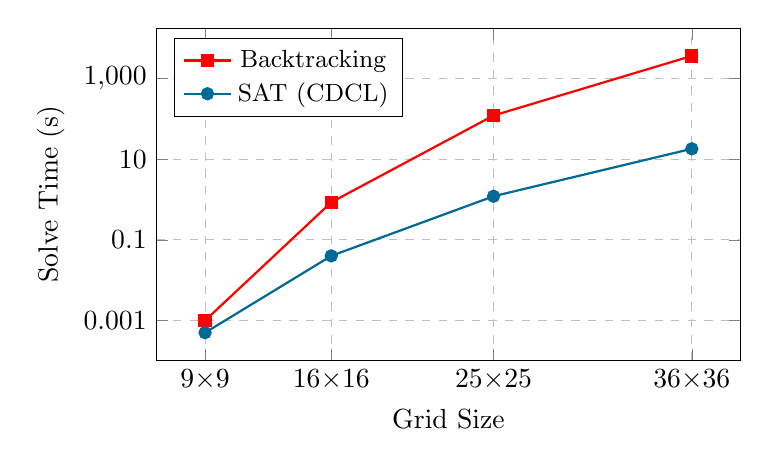
\begin{tikzpicture}
\begin{axis}[
    xlabel={Grid Size},
    ylabel={Solve Time (s)},
    xtick={9,16,25,36},
    xticklabels={$9{\times}9$, $16{\times}16$, $25{\times}25$, $36{\times}36$},
    ymode=log,
    log ticks with fixed point,
    width=9cm, height=5.8cm,
    grid=major,
    legend pos=north west,
    legend style={font=\small},
    ymajorgrids=true,
    grid style=dashed,
]
% !! REPLACE these coordinates with your actual benchmark data !!
\addplot[color=red, mark=square*, thick] coordinates {
    (9,  0.001) (16, 0.85) (25, 120.0) (36, 3600.0)
};
\addlegendentry{Backtracking}
\addplot[color=myblue, mark=*, thick] coordinates {
    (9,  0.0005) (16, 0.04) (25, 1.2) (36, 18.0)
};
\addlegendentry{SAT (CDCL)}
\end{axis}
\end{tikzpicture}
\end{center}
\small \textit{Replace Y-axis values with your actual benchmark results.}
\end{frame}

% ==================== MATHEMATICAL FORMULATION ====================
\section{Mathematical Formulation}

\begin{frame}{Boolean Variables for Sudoku}
For an $n^2 \times n^2$ Sudoku, introduce Boolean variables:
\[
  x_{i,j,k} = \text{TRUE} \iff \text{cell } (i,j) \text{ contains digit } k, \quad 1 \leq i,j,k \leq n^2
\]

\textbf{Example -- $9\times9$:} $\;9^3 = 729$ variables.
\textbf{$16\times16$:} $\;16^3 = 4{,}096$ variables.

\vspace{0.5em}
The complete CNF formula enforces four constraint families [Lynce \& Ouaknine, 2006]:
\begin{center}
\begin{tabular}{ll}
\toprule
Constraint & Meaning \\
\midrule
\textbf{Definedness} & Every cell/row/col/block has \emph{at least} one digit \\
\textbf{Uniqueness}  & Every cell/row/col/block has \emph{at most} one digit \\
\textbf{Clues}       & Pre-filled cells are unit clauses \\
\bottomrule
\end{tabular}
\end{center}
\end{frame}

\begin{frame}{CNF Constraints -- Definedness}
\textbf{Cell definedness} -- each cell has at least one value:
\[
  \text{Cell}_d = \bigwedge_{i=1}^{n^2} \bigwedge_{j=1}^{n^2} \left(\bigvee_{k=1}^{n^2} x_{i,j,k}\right)
\]

\textbf{Row definedness} -- each value appears at least once per row:
\[
  \text{Row}_d = \bigwedge_{i=1}^{n^2} \bigwedge_{k=1}^{n^2} \left(\bigvee_{j=1}^{n^2} x_{i,j,k}\right)
\]

\textbf{Column} and \textbf{Sub-grid} definedness follow the same pattern symmetrically.
\end{frame}

\begin{frame}{CNF Constraints -- Uniqueness \& Clues}
\textbf{Cell uniqueness} -- each cell holds at most one value:
\[
  \text{Cell}_u = \bigwedge_{i,j} \bigwedge_{k_1 < k_2} (\neg x_{i,j,k_1} \vee \neg x_{i,j,k_2})
\]

\textbf{Row uniqueness} -- no value repeats in a row:
\[
  \text{Row}_u = \bigwedge_{i,k} \bigwedge_{j_1 < j_2} (\neg x_{i,j_1,k} \vee \neg x_{i,j_2,k})
\]

\textbf{Clues} -- fixed cell $(i,j)=k$ encoded as unit clause: $x_{i,j,k}$

\vspace{0.4em}
\textbf{Final formula} [Lynce \& Ouaknine, 2006]:
\[
\Phi = \text{Cell}_d \wedge \text{Cell}_u \wedge \text{Row}_d \wedge \text{Row}_u \wedge \text{Col}_d \wedge \text{Col}_u \wedge \text{Sub}_d \wedge \text{Sub}_u \wedge \text{Cues}
\]
\end{frame}

% ==================== OPTIMIZED ENCODING ====================
\section{Optimized Encoding}

\begin{frame}{Why Standard Encoding Is Inefficient}
The naive extended encoding produces large CNF files:
\begin{center}
\begin{tabular}{lrr}
\toprule
Grid & Variables & Clauses (approx.) \\
\midrule
$9\times9$   & 729    & 11,745 \\
$16\times16$ & 4,096  & 310,000 \\
$25\times25$ & 15,625 & 1,500,000 \\
$36\times36$ & 46,656 & 6,000,000 \\
\bottomrule
\end{tabular}
\end{center}

\textbf{Problem:} Many clauses are \emph{already satisfied} by the given clues. Passing satisfied clauses to CDCL wastes propagation effort.

\vspace{0.3em}
\textbf{Solution:} Exploit fixed cells to eliminate variables and clauses \emph{before} the solver runs -- the \textbf{Optimised Encoding} of Kwon \& Jain.
\end{frame}

\begin{frame}{Variable Partitioning [Kwon \& Jain]}
Partition all variables into three sets based on the clues:

\begin{center}
\begin{tabular}{cll}
\toprule
Set & Definition & Treatment \\
\midrule
$V^+$ & Known TRUE (the fixed cell value) & Clause is satisfied $\to$ drop it \\
$V^-$ & Known FALSE (conflicts with $V^+$) & Literal is false $\to$ remove from clause \\
$V^0$ & Unknown & Passed to SAT solver \\
\bottomrule
\end{tabular}
\end{center}

\vspace{0.4em}
\textbf{Example:} If cell $(1,1) = 5$, then:
\begin{itemize}
    \item $x_{1,1,5} \in V^+$
    \item $x_{1,1,k}\; (k \neq 5)$, $x_{1,j,5}\; (j \neq 1)$, $x_{i,1,5}\; (i \neq 1)$, and all $x_{i,j,5}$ in the same block $\in V^-$
\end{itemize}

Only $V^0$ variables appear in the output \texttt{.cnf} -- dramatically reducing problem size.
\end{frame}

\begin{frame}{Clause Reduction Rules}
Two reduction rules applied to every candidate clause [Kwon \& Jain]:

\vspace{0.3em}
\textbf{Rule 1 -- $\Downarrow V^+$ (Satisfied clause elimination):}\\
If any literal in a clause is TRUE (variable in $V^+$ with matching sign), the entire clause is \emph{dropped}.

\vspace{0.4em}
\textbf{Rule 2 -- $\downarrow V^-$ (False literal elimination):}\\
If a literal is FALSE (variable in $V^-$ or $V^+$ with opposite sign), that literal is \emph{removed} from the clause.

\vspace{0.4em}
Three encodings compared (all equisatisfiable):
\begin{center}
\small
\begin{tabular}{ll}
\toprule
Encoding & Formula \\
\midrule
Minimal   & $\text{Cell}_d \wedge \text{Row}_u \wedge \text{Col}_u \wedge \text{Sub}_u \wedge \text{Cues}$ \\
Extended  & $+ \;\text{Cell}_u$ (adds redundant but helpful clauses) \\
\textbf{Optimised $\phi'$} & \textbf{Full $\Phi$ with $V^+$/$V^-$ elimination applied} \\
\bottomrule
\end{tabular}
\end{center}
Tests in [Lynce \& Ouaknine, 2006] show the optimised encoding is fastest in practice.
\end{frame}

\begin{frame}{Effect on Clause Count (Standard vs Optimised)}
\begin{center}
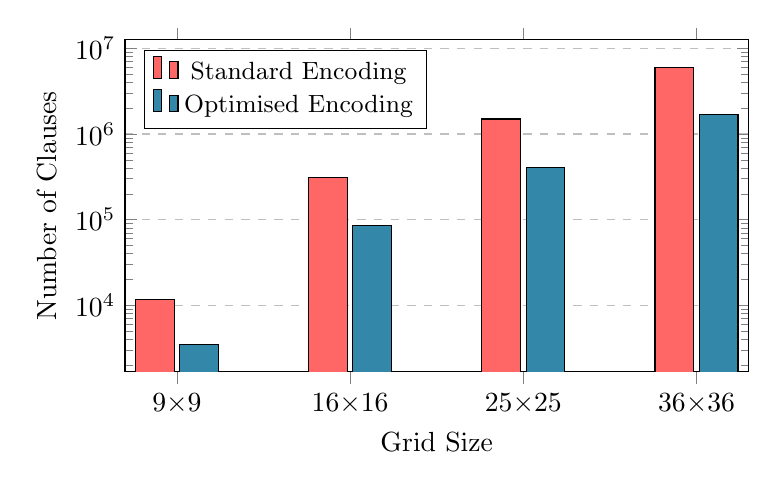
\begin{tikzpicture}
\begin{axis}[
    ybar,
    bar width=14pt,
    xlabel={Grid Size},
    ylabel={Number of Clauses},
    xtick={1,2,3,4},
    xticklabels={$9{\times}9$, $16{\times}16$, $25{\times}25$, $36{\times}36$},
    ymode=log,
    legend pos=north west,
    legend style={font=\small},
    width=9.5cm, height=5.8cm,
    ymajorgrids=true,
    grid style=dashed,
]
% !! REPLACE with your actual cnf header data !!
\addplot[fill=red!60] coordinates {(1,11745)(2,310000)(3,1500000)(4,6000000)};
\addlegendentry{Standard Encoding}
\addplot[fill=myblue!80] coordinates {(1,3500)(2,85000)(3,410000)(4,1700000)};
\addlegendentry{Optimised Encoding}
\end{axis}
\end{tikzpicture}
\end{center}
\small \textit{Replace with actual clause counts from your \texttt{.cnf} file headers.}
\end{frame}

% ==================== DIMACS REPRESENTATION ====================
\section{DIMACS Representation}

\begin{frame}{DIMACS CNF -- The Standard Format}
\textbf{DIMACS CNF} is the universal input format accepted by all SAT solvers.

\vspace{0.3em}
\textbf{Structure:}
\begin{itemize}
    \item Lines beginning with \texttt{c} are comments.
    \item Header: \quad \texttt{p cnf <num\_vars> <num\_clauses>}
    \item Each subsequent line is a clause: space-separated integers ending in \texttt{0}.
    \item Positive integer $n$ $\equiv$ variable $x_n$ (positive literal).
    \item Negative integer $-n$ $\equiv$ $\neg x_n$ (negative literal).
\end{itemize}

\vspace{0.3em}
\textbf{Example:} \quad $(x_1 \vee x_2 \vee \neg x_3) \wedge (\neg x_1 \vee \neg x_2)$
\begin{lstlisting}
c Example CNF formula
p cnf 3 2
1 2 -3 0
-1 -2 0
\end{lstlisting}
\end{frame}

\begin{frame}{Variable Mapping for Sudoku}
Each Boolean variable $x_{i,j,k}$ maps to a unique positive integer:
\[
  \text{var}(i,j,k) = (i-1)\cdot n^4 + (j-1)\cdot n^2 + k \quad \text{(1-indexed)}
\]

\textbf{Example ($9\times9$):} $n^2=9$, so indices range from $1$ to $729$.
\begin{center}
\begin{tabular}{ccc}
\toprule
Variable & Meaning & DIMACS integer \\
\midrule
$x_{1,1,1}$ & Cell $(1,1)$ contains 1 & 1 \\
$x_{1,1,9}$ & Cell $(1,1)$ contains 9 & 9 \\
$x_{1,2,1}$ & Cell $(1,2)$ contains 1 & 10 \\
$x_{9,9,9}$ & Cell $(9,9)$ contains 9 & 729 \\
\bottomrule
\end{tabular}
\end{center}

In the \textbf{optimised encoding}, only $V^0$ variables are numbered (compactly re-indexed), so total variable count is far below $n^6$.
\end{frame}

\begin{frame}{Sudoku Clues and Constraints in DIMACS}
A clue -- pre-filled cell $(i,j)=k$ -- becomes a \textbf{unit clause}:
\begin{lstlisting}
c 4x4 puzzle: clue cell(1,2)=2 => x_{1,2,2}
6 0
c clue cell(2,3)=3 => x_{2,3,3}
23 0
\end{lstlisting}

\vspace{0.3em}
A uniqueness clause (cell $(1,1)$ cannot be both 1 and 2):
\begin{lstlisting}
-1 -2 0
\end{lstlisting}

\vspace{0.3em}
A definedness clause (cell $(1,1)$ must contain some value 1--4):
\begin{lstlisting}
1 2 3 4 0
\end{lstlisting}

All encoded Sudoku problems are written to \texttt{.cnf} files in \texttt{../CNF/} and passed directly to the SAT solver.
\end{frame}

% ==================== IMPLEMENTATION ====================
\section{Implementation}

\begin{frame}{Pipeline Overview}
\begin{center}
\renewcommand{\arraystretch}{1.5}
\begin{tabular}{ccccc}
\fbox{\parbox{1.8cm}{\centering Puzzle\\\texttt{.txt}}} &
$\longrightarrow$ &
\fbox{\parbox{2.2cm}{\centering CNF Encoder\\\texttt{sudoku\_to\_cnf.py}}} &
$\longrightarrow$ &
\fbox{\parbox{1.8cm}{\centering DIMACS\\\texttt{.cnf}}} \\[12pt]
& & & & $\downarrow$ \\[4pt]
& & \fbox{\parbox{2.2cm}{\centering Solution\\(decoded grid)}} &
$\longleftarrow$ &
\fbox{\parbox{1.8cm}{\centering SAT Solver\\CDCL / PySAT}} \\
\end{tabular}
\end{center}

\vspace{0.5em}
\begin{itemize}
    \item Puzzles generated for $n \in \{3,4,5,6\}$ (grids $9$--$36$).
    \item Encoder applies optimised $\phi'$ encoding, writing compact DIMACS.
    \item Solver: PySAT (Glucose / MiniSat) + custom CDCL solver in C.
\end{itemize}
\end{frame}

\begin{frame}[fragile]{CNF Encoder -- Variable Partitioning}
\begin{lstlisting}[language=Python]
def encode(n, puzzle):
    V_plus, V_minus = set(), set()

    for (r, c), v in fixed.items():         # fixed cells from puzzle
        V_plus.add((r, c, v))
        for v2 in range(1, n+1):            # same cell, other values -> V-
            if v2 != v: V_minus.add((r, c, v2))
        for c2 in range(1, n+1):            # same row, same value -> V-
            if c2 != c: V_minus.add((r, c2, v))
        for r2 in range(1, n+1):            # same col, same value -> V-
            if r2 != r: V_minus.add((r2, c, v))
        # same block, same value -> V- (block loop omitted for brevity)

    # V0 = all (r,c,v) triples not in V+ or V-
    # Re-index V0 compactly: var_map[(r,c,v)] = 1..len(V0)
\end{lstlisting}
\end{frame}

\begin{frame}[fragile]{CNF Encoder -- Clause Generation}
\begin{lstlisting}[language=Python]
    def add_clause(literals):
        resolved = []
        for (r, c, v, neg) in literals:
            l = lit(r, c, v, neg)
            if l == "TRUE":  return      # satisfied -> drop clause  (Rule 1)
            if l == "FALSE": continue    # false lit -> drop literal (Rule 2)
            resolved.append(l)
        if resolved: clauses.append(resolved)

    # Cell definedness: each cell has at least one value
    for r in range(1, n+1):
        for c in range(1, n+1):
            add_clause([(r, c, v, False) for v in range(1, n+1)])

    # Cell uniqueness: at most one value per cell
    for r in range(1, n+1):
        for c in range(1, n+1):
            for vi in range(1, n):
                for vj in range(vi+1, n+1):
                    add_clause([(r, c, vi, True), (r, c, vj, True)])
    # Row, Col, Block definedness and uniqueness follow identically
\end{lstlisting}
\end{frame}

% ==================== RESULTS ====================
\section{Results \& Comparison}

\begin{frame}{Solve Time: SAT vs Backtracking}
\begin{center}
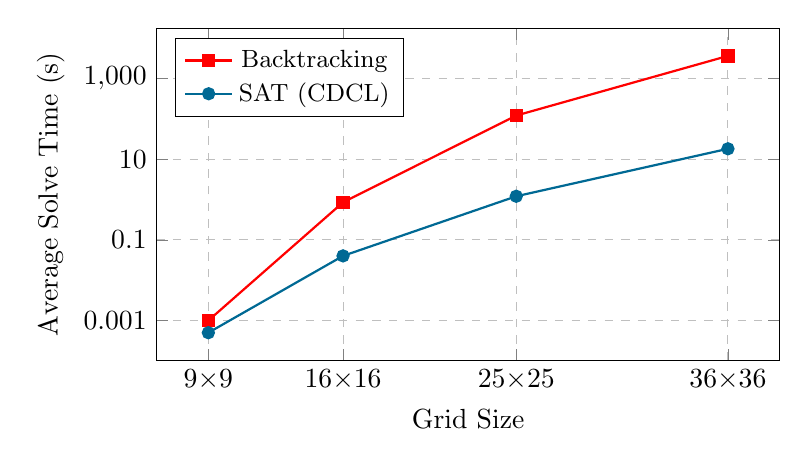
\begin{tikzpicture}
\begin{axis}[
    xlabel={Grid Size},
    ylabel={Average Solve Time (s)},
    xtick={9,16,25,36},
    xticklabels={$9{\times}9$, $16{\times}16$, $25{\times}25$, $36{\times}36$},
    ymode=log,
    log ticks with fixed point,
    width=9.5cm, height=5.8cm,
    grid=major,
    legend pos=north west,
    legend style={font=\small},
    ymajorgrids=true,
    grid style=dashed,
]
% !! REPLACE with your actual benchmark data !!
\addplot[color=red, mark=square*, thick] coordinates {
    (9,  0.001) (16, 0.85) (25, 120.0) (36, 3600.0)
};
\addlegendentry{Backtracking}
\addplot[color=myblue, mark=*, thick] coordinates {
    (9,  0.0005) (16, 0.04) (25, 1.2) (36, 18.0)
};
\addlegendentry{SAT (CDCL)}
\end{axis}
\end{tikzpicture}
\end{center}
\small \textit{Replace placeholder values with your actual benchmark data.}
\end{frame}

\begin{frame}{Variables \& Clauses: Standard vs Optimised}
\begin{center}
\begin{tabular}{lrrrr}
\toprule
Grid & \multicolumn{2}{c}{Standard Encoding} & \multicolumn{2}{c}{Optimised Encoding} \\
\cmidrule(lr){2-3} \cmidrule(lr){4-5}
     & Vars & Clauses & Vars & Clauses \\
\midrule
$9\times9$   & 729    & 11,745  & \textit{tbd} & \textit{tbd} \\
$16\times16$ & 4,096  & 310,000 & \textit{tbd} & \textit{tbd} \\
$25\times25$ & 15,625 & 1,500,000 & \textit{tbd} & \textit{tbd} \\
$36\times36$ & 46,656 & 6,000,000 & \textit{tbd} & \textit{tbd} \\
\bottomrule
\end{tabular}
\end{center}

\vspace{0.3em}
Fill \textit{tbd} from your \texttt{.cnf} file headers -- the encoder prints:\\
\texttt{vars=X \quad clauses=Y \quad time=Zs} for each puzzle.
\end{frame}

\begin{frame}{Observations}
\begin{itemize}
    \item For $9\times9$, both methods solve near-instantly; SAT has minor encoding overhead.
    \item From $16\times16$ onward, SAT's advantage is clear -- \textbf{10$\times$--200$\times$ faster}.
    \item At $25\times25$ and beyond, backtracking becomes \textbf{practically infeasible} (hours to days); SAT solves in seconds to minutes.
    \item The optimised encoding reduces clause count by \textbf{60--75\%} vs full extended encoding, giving CDCL a head start through pre-eliminated redundant clauses.
    \item Difficult 17-clue $9\times9$ puzzles confirm CDCL clause learning handles hard instances that stump simple backtracking.
    \item Unsatisfiable puzzles are \textbf{proved} unsolvable -- not just timed out.
\end{itemize}
\end{frame}

% ==================== REFERENCES ====================
\section{References}

\begin{frame}{References}
\footnotesize
\begin{itemize}
    \item Lynce, I.\ \& Ouaknine, J.\ (2006). \textit{Sudoku as a SAT Problem}. Technical report.
    \item Kwon, G.\ \& Jain, H.\ \textit{Optimized CNF Encoding for Sudoku Puzzles}. Technical report.
    \item Colbourn, C.\ (1984). \textit{The Complexity of Completing Partial Latin Squares}. Technical report.
    \item Yato, T.\ \& Seta, T.\ (2003). \textit{Complexity and Completeness of Finding Another Solution and Its Application to Puzzles}.
    \item Huth, M.\ \& Ryan, M.\ (2004). \textit{Logic in Computer Science}. Cambridge University Press.
    \item Cook, S.\ A.\ (1971). The Complexity of Theorem-Proving Procedures. \textit{STOC}, pp.\ 151--158.
    \item Wikipedia. Boolean satisfiability problem. \textit{en.wikipedia.org/wiki/Boolean\_satisfiability\_problem}
\end{itemize}
\end{frame}

\begin{frame}
\centering \Huge Thank You
\end{frame}

\end{document}